\documentclass[11pt,letterpaper]{article}

% --- layout & typography ---
\usepackage[margin=1in]{geometry}
\usepackage{microtype}
\usepackage[T1]{fontenc}
\usepackage{lmodern}

% --- math & symbols ---
\usepackage{amsmath,amssymb,amsfonts}
\usepackage{siunitx}
\usepackage{xspace}
\usepackage{mathtools}

% --- graphics & tables ---
\usepackage{graphicx}
\usepackage{booktabs}
\usepackage{array}
\usepackage{tabularx}             % flexible-width tables
\usepackage[section]{placeins}    % keep floats within their section
\usepackage{tcolorbox}            % for design card
\usepackage{enumitem}             % compact lists

% --- links (load hyperref near last) ---
\usepackage{xcolor}
\usepackage{hyperref}
\hypersetup{
  colorlinks=true,
  linkcolor=blue!50!black,
  citecolor=blue!50!black,
  urlcolor=blue!50!black
}

% --- optional: smarter refs (after hyperref) ---
\usepackage[nameinlink]{cleveref}

% --- identifiers / config ---
\newcommand{\confighash}{c7dc5aa1}

% --- robust, math-safe macros ---
\DeclareRobustCommand{\mrl}{\textsc{MRL}\xspace}
\DeclareRobustCommand{\mrc}{\textbf{MRC}\xspace}
\DeclareRobustCommand{\classS}{\textbf{Class~S}\xspace}
\DeclareRobustCommand{\classC}{\textbf{Class~C}\xspace}
\DeclareRobustCommand{\classM}{\textbf{Class~M}\xspace}
\DeclareRobustCommand{\GatePSD}{\ensuremath{\text{PSD-NRMSE}<0.03}\xspace}
\DeclareRobustCommand{\GateDZ}{\ensuremath{\lvert d_z\rvert<0.30}\xspace}
\DeclareRobustCommand{\GateEQ}{\ensuremath{\GatePSD \wedge \GateDZ}\xspace}

% --- tabularx helpers: ragged X columns ---
\newcolumntype{Y}{>{\raggedright\arraybackslash}X}

% --- title block ---
\title{\bfseries\Large
The Memory-Resonance Condition ($\Theta\!\approx\!1$): A mechanism-aware design rule with diagnostics and a minimal testbed\\[0.35em]
\itshape\normalsize
Timescale matching as a widely recurring control principle}
\author{[Mat Thompson, \emph{Independent Researcher}]}
\date{\today}

\begin{document}
\maketitle

\begin{abstract}
Across domains---from stochastic resonance in neural circuits to noise-assisted quantum transport---systems exhibit enhanced performance when environmental memory matches their fastest internal rhythm. We recognize this cross-domain pattern as a unified phenomenon and formalize it as the \emph{Memory-Resonance Condition} (\mrc): $\Theta \equiv \omega_{\mathrm{fast}}\tau_B \approx 1$, where $\tau_B$ is the bath correlation time and $\omega_{\mathrm{fast}}$ is the dominant transduction frequency. The \emph{observable} (a shallow optimum near $\Theta\!\approx\!1$) recurs across substrates; the \emph{mechanism} varies. We propose a taxonomy: \classS{} (spectral overlap in linear systems), \classC{} (coherent modulation via weak nonlinearity), and \classM{} (memory backaction from time-nonlocal kernels). To operationalize this classification, we introduce two diagnostic controls---a PSD-matched surrogate (tests \classS) and an equal-carrier calibration (tests \classM)---and validate with a minimal three-mode hierarchy. Classical pillar: Ornstein--Uhlenbeck (OU) and phase-randomized surrogates are practically equivalent (PSD-NRMSE$<$0.03, $|d_z|<$0.30), confirming spectral overlap dominates (\classS). Quantum pillar: equal-carrier scans retain $\Theta\!\approx\!1$ structure despite fixed spectral weight at $\omega_1$ ($|\Delta J|/J^\star\!\le\!0.02$), consistent with memory backaction (\classM). The \mrc unifies scattered observations into an actionable design rule: \emph{tune environmental memory toward resonance with internal dynamics}.
\end{abstract}

\section{Introduction}
A recurring observation across physics, biology, and engineering is that \emph{finite-memory} noise can improve function when its correlation time $\tau_B$ is commensurate with an internal timescale. Examples span stochastic/coherence resonance, noise-assisted transport, neural detection under colored noise, and energy harvesting. Despite different substrates---classical damped oscillators, quantum transport networks, excitable neural circuits, photosynthetic complexes---a common functional form emerges: performance peaks near $\Theta\equiv\omega_{\mathrm{fast}}\tau_B\approx 1$, where $\omega_{\mathrm{fast}}$ is the system's dominant transduction frequency and $\tau_B$ is the environmental correlation time.

\emph{Why does the same shape recur?} In this work we recognize this as a \emph{unified phenomenon} and formalize it as the Memory-Resonance Condition (\mrc). Our synthesis perspective reveals that: (i) the \emph{observable} (a shallow interior optimum near $\Theta\!\approx\!1$) is generic across substrates, appearing whenever environmental memory synchronizes with internal dynamics; (ii) the \emph{mechanism} varies---spectral overlap in near-linear systems (\classS), coherent modulation under weak nonlinearity (\classC), memory backaction from time-nonlocal kernels (\classM); and (iii) these mechanisms are \emph{operationally distinguishable} via controlled comparisons. The value of the \mrc is that it converts scattered domain-specific observations into a predictive control law: tune $\tau_B$ toward $1/\omega_{\mathrm{fast}}$ to maximize performance, then diagnose which mechanism is operative.

We \textbf{do not} claim novelty of the phenomenon; our contribution is an \emph{operational design rule} and \emph{diagnostics} that make it testable and tunable. We connect to prior work---stochastic resonance (Gammaitoni et al.), coherence resonance (Pikovsky \& Kurths), resonant activation, noise-assisted transport---which exhibit similar timescale-matching phenotypes but with substrate-specific mechanisms.

To make these classes \emph{operationally testable}, we introduce two controls that factor mechanisms: (1) a \emph{PSD-matched surrogate} replaces temporal phases while preserving the drive spectrum (tests \classS); (2) a \emph{quantum equal-carrier} calibration holds the fast-mode spectral weight fixed while scanning $\tau_B$ (tests \classM). We validate with a minimal three-mode hierarchy computed in the \emph{frequency} domain using identical windows for classical and quantum paths. The experiments are supplementary: their role is to operationalize the taxonomy and show how to diagnose which class applies in practice.

\paragraph*{Terminology.} We use \textbf{MRC} (Memory-Resonance \emph{Condition}, $\Theta\!\approx\!1$), the \textbf{MR line} ($\Theta=1$ reference), and the \textbf{MR band} (practical optimum window, here $[0.7,1.4]$). We plot and reason in terms of the \emph{band}, not a razor line.

\section{Synthesis map and taxonomy}
Table~\ref{tab:crossdomain} summarizes representative reports of timescale-matching optima across domains. We group mechanisms into \classS{}, \classC{}, and \classM{} based on which control nulls the effect. This perspective is akin to universality classes: the \emph{phenotype} (an interior optimum near $\Theta\!\approx\!1$) is shared, while the \emph{micro-mechanism} differs. The value of the \mrc is pragmatic: it is a \emph{tunable control law} that remains useful regardless of mechanism, provided one runs the appropriate controls to identify the class.

\begin{table}[h!]
\centering
\caption{Representative cross-domain observations of timescale matching.}
\label{tab:crossdomain}
\begin{tabularx}{\linewidth}{@{}lYYl@{}}
\toprule
Domain & System & Matching & Reference \\
\midrule
Classical SR & Damped oscillator + colored noise & $\omega_0 \tau_B \approx 1$ & Mondal et al. (2018) \cite{Mondal2018} \\
Excitable circuits & FitzHugh--Nagumo + colored noise & Coherence peak at optimal $\tau_B$ & Brugioni et al. (2005) \cite{Brugioni2005} \\
Quantum transport & Network + correlated dephasing & Enhanced transport at finite $\tau_B$ & Moreira et al. (2020) \cite{Moreira2020} \\
Neural detection & Threshold neurons + colored noise & Optimal SNR at intermediate $\tau_B$ & Duan et al. (2014) \cite{Duan2014} \\
Energy harvesting & Oscillator chain + colored noise & Peak power at matched bandwidth & Romero-Bastida \& L\'opez (2020) \cite{RomeroBastida2020} \\
Photosynthesis & Exciton network + structured bath & Noise-assisted transport & Uchiyama et al. (2017) \cite{Uchiyama2017} \\
\bottomrule
\end{tabularx}
\end{table}

\clearpage
\section{Framework: overlap functional and classes}
Let $H_{n\leftarrow\xi}(\omega)$ denote the transfer from bath $\xi$ to a slow node $n$ and let $S_\xi(\omega;\tau_B)$ be the bath PSD. Define the slow-band objective
\begin{equation}
J(\tau_B) = \int_{\Omega_{\rm slow}} \big|H_{n\leftarrow\xi}(\omega)\big|^2\, S_\xi(\omega;\tau_B)\, \mathrm{d}\omega,
\end{equation}
with $\Omega_{\rm slow}$ a band around $\omega_n$. \emph{For Class S (LTI systems), this reduces to the standard output variance formula via the Wiener-Khinchin theorem}: the steady-state response variance is the integral of the power spectral density weighted by the squared system gain. Under timescale separation and a dominant lobe near $\omega_{\rm fast}$, $J(\tau_B)$ typically exhibits a shallow interior optimum when the bath peak aligns with this lobe, yielding $\Theta \equiv \omega_{\mathrm{fast}} \tau_B \approx 1$. We term this the \emph{Memory-Resonance Condition}. The MRC generalizes this frequency-domain bandwidth-matching principle beyond linear systems to Classes C and M, where the functional form persists but the underlying mechanism differs.

\paragraph{Why an interior maximum?}
For OU noise with fixed power $D$ and $S_{\rm OU}(\omega;\kappa) = 2D\kappa/(\omega^2+\kappa^2)$, short $\tau_B$ ($\kappa$ large) spreads power across all frequencies but dilutes it at $\omega_{\rm fast}$. Long $\tau_B$ ($\kappa$ small) concentrates power near DC, missing the system's peak gain at $\omega_{\rm fast}$. The optimum arises from the product $|H|^2 S$: increasing $\tau_B$ narrows the bath spectrum (raising $S$ at low $\omega$), but the system gain $|H(\omega)|^2$ peaks elsewhere. Maximum overlap occurs when the bath centroid $\sim 1/\tau_B$ aligns with the system's dominant transduction frequency $\omega_{\rm fast}$, hence $\omega_{\rm fast} \tau_B \approx 1$. This interior trade-off is \emph{not} universal---heavily multi-peaked $H(\omega)$ or power-law baths can yield monotonic curves---but recurs widely under single-lobe + timescale-separation conditions.

We distinguish mechanisms by controls:
\begin{itemize}
\item \classS: LTI response; PSD-matched surrogate (preserve magnitude, randomize phases) yields equivalence $\Rightarrow$ spectral mechanism.
\item \classC: weakly nonlinear/modulated; coherence redistributes spectral weight.
\item \classM: equal-carrier (hold $J(\omega_1)$ fixed across $\kappa=1/\tau_B$). Persisting $\Theta$-structure $\Rightarrow$ memory/backaction.
\end{itemize}

\section{Metrics, controls, and gates}
\paragraph*{Operational definitions.}
We define the system's fast scale $\omega_{\mathrm{fast}}$ as the dominant frequency at which fluctuations at the coupling interface are most efficiently transduced into the measured (slow-band) observable. Concretely:

\emph{Linear/near-linear:} $\omega_{\mathrm{fast}} := \arg\max_{\omega} |H_{\mathrm{slow}\leftarrow\mathrm{int}}(\omega)|^2$, where $H_{\mathrm{slow}\leftarrow\mathrm{int}}$ is the transfer from the bath interface to the measured channel.

\emph{Nonlinear (operating point):} Linearize the dynamics around the operating state; take the eigenfrequency whose right singular vector has the largest projection onto the measured channel.

\emph{Periodically driven:} Use the leading Floquet rate (dominant quasi-energy with nonzero projection onto the measured channel).

We report the chosen mode and include a sensitivity analysis when multiple candidates are comparable (quantitative threshold: if $|H(\omega_1)|^2 / |H(\omega_2)|^2 > 3$, use $\omega_1$ as dominant; else report sensitivity to both). \emph{Our testbed:} In the three-oscillator hierarchy, $\omega_{\mathrm{fast}}=\omega_1=1.0\,\mathrm{rad/s}$ (dominant peak in $|H_{\omega_3\leftarrow\mathrm{bath}}(\omega)|^2$).

\paragraph*{Timescale separation criterion.}
The MRC assumes separation between fast transduction ($\omega_{\mathrm{fast}}$) and slow observable ($\omega_{\mathrm{slow}}$). We adopt: \emph{Strong separation} ($\omega_{\mathrm{fast}}/\omega_{\mathrm{slow}} > 5$, MRC applies); \emph{Weak separation} ($1 < \omega_{\mathrm{fast}}/\omega_{\mathrm{slow}} \le 5$, MRC may apply with caution); \emph{No separation} ($\omega_{\mathrm{fast}}/\omega_{\mathrm{slow}} \le 1$, MRC not applicable). In our hierarchy, $\omega_1/\omega_3 = 10$, ensuring strong separation.

\paragraph*{Bath correlation times.}
We use two complementary definitions:

\emph{Bath-intrinsic correlation time} (system-independent):
\[
\tau_B^{(\mathrm{int})} := \int_0^\infty \frac{C_\xi(\tau)}{C_\xi(0)}\,\mathrm{d}\tau,
\]
whenever the autocorrelation $C_\xi(\tau)=\langle\xi(t)\xi(t-\tau)\rangle$ exists and is integrable.

\emph{Observable-effective correlation time} (predictive for the measured channel):
\[
\tau_B^{(\mathrm{eff})} := \frac{1}{2\pi f_{\mathrm{char}}},\quad
f_{\mathrm{char}} = \frac{\int_0^\infty \omega\, |H(\omega)|^2 S_\xi(\omega)\,\mathrm{d}\omega}
{\int_0^\infty |H(\omega)|^2 S_\xi(\omega)\,\mathrm{d}\omega}.
\]
$\tau_B^{(\mathrm{eff})}$ weights spectral content by the system's gain and is what the design rule uses to predict performance for the \emph{measured} observable. For OU noise with decay rate $\kappa$, we have $\tau_B^{(\mathrm{int})}=\tau_B^{(\mathrm{eff})}=1/\kappa$ (validated by comparing autocorrelation integral to spectral centroid; agreement within 2\%). Unless otherwise specified, we report both values (with CIs) and verify that they agree within tolerance.

\paragraph*{Metrics (shared, frequency domain).}
We use (i) baseband variance after I/Q demodulation via a 4th-order Butterworth low-pass around $f_3=\omega_3/2\pi$; (ii) narrowband PSD power over $[f_3(1-\beta),f_3(1+\beta)]$ (default $\beta=0.30$). Spectra are one-sided densities.

\paragraph*{Classical control (\classS).}
We compare OU input to its PSD-matched surrogate: preserve rFFT magnitudes, randomize phases (DC/Nyquist $=0$), inverse transform, restore the mean. Statistics are \emph{paired} across seeds. We adopt \emph{practical-equivalence} gates: \GateEQ{} at each $\Theta$. \emph{Rationale for thresholds}: PSD-NRMSE$<$0.03 ensures spectral differences are below typical measurement noise in experimental setups (3\% is standard in calibration protocols); $|d_z|<$0.30 corresponds to Cohen's ``small'' effect size, ensuring detected differences are not just statistically significant but also practically negligible relative to the $\Theta$-dependence itself (which exhibits $d_z\!\sim\!1$--$2$ between MR band and boundaries). Paired Cohen's $d_z$ (effect size for paired comparisons, $d_z=t/\sqrt{n}$) and Holm-adjusted $p$ are \emph{reported} but \emph{not gated}. \emph{Normalization:} total variance equalized across $\Theta$; integrated power matched over $[\omega_{\mathrm{fast}}/\sqrt{10},\sqrt{10}\,\omega_{\mathrm{fast}}]$. \emph{Spectral estimation:} Welch's method with Hann window, 50\% overlap, segment length chosen to ensure $\ge 16$ segments per realization.

\paragraph*{Quantum control (\classM).}
We enforce \emph{equal-carrier}: hold $J(\omega_1)$ fixed while scanning $\kappa=1/\tau_B$. Calibration uses a Lorentzian ansatz with short refine; points failing $|\Delta J|/J^\star\le 0.02$ are rejected. We set the calibration bandwidth fraction to zero (\texttt{j\_bandwidth\_frac=0}) to ensure the bath spectral weight is concentrated exactly at $\omega_1$. Curves are computed with a Gaussian covariance solver (continuous Lyapunov equation): we solve $A\Sigma + \Sigma A^\dagger = -D$ for the steady-state covariance $\Sigma$, where $A$ is the drift matrix of the Gaussian master equation and $D$ is the diffusion matrix. \emph{Stability condition}: All eigenvalues of $A$ satisfy $\Re\lambda < 0$ (Lyapunov stability, ensures exponential relaxation to steady state); we enforce $\min\Re\lambda(A) < -10^{-6}$ as a numerical safety margin. A trajectory engine is retained for \emph{parity} and matches within $10^{-3}$ at $\Theta=0.95$.

\paragraph*{Reproducibility and QA.}
Each row carries a UTC timestamp, run UUID, solver, wallclock, and (quantum) $\min \Re \lambda(A)$ and SPD checks. A single consolidated CSV drives all figures (config hash \texttt{\confighash}). QA gates: stability + SPD (quantum), equal-carrier tolerance, and \GateEQ{} (classical).

\begin{tcolorbox}[colback=blue!5!white,colframe=blue!75!black,title=Design Card: Memory-Resonance Condition ($\Theta \approx 1$)]

\paragraph*{Rule.} Target $\Theta \equiv \omega_{\mathrm{fast}} \tau_B$ in the \textbf{MR band} $[0.7, 1.4]$ (treat as window, not razor line).

\paragraph*{Estimate $\omega_{\mathrm{fast}}$:}
\begin{itemize}[nosep,leftmargin=*]
\item \emph{Linear/near-linear:} $\arg\max_\omega |H_{\mathrm{slow}\leftarrow\mathrm{int}}(\omega)|^2$
\item \emph{Nonlinear:} Linearize at operating point; pick eigenmode with largest projection onto slow observable
\item \emph{Periodically driven:} Leading Floquet rate with nonzero projection
\end{itemize}

\paragraph*{Select $\tau_B$:}
Use the \emph{observable-effective} timescale $\tau_B^{(\mathrm{eff})}$ (spectral centroid weighted by system gain), not bath-intrinsic $\tau_B^{(\mathrm{int})}$ (autocorr integral), if they differ.

\paragraph*{Diagnostics (Mechanism Class):}
\begin{itemize}[nosep,leftmargin=*]
\item \textbf{Class S} (Spectral overlap): PSD-matched surrogate reproduces optimum
\item \textbf{Class C} (Coherent modulation): Surrogate fails; equal-carrier scan is flat
\item \textbf{Class M} (Memory backaction): Surrogate fails; equal-carrier scan retains $\Theta\!\approx\!1$ structure
\end{itemize}

\paragraph*{Failure modes:}
Heavy-tail baths ($1/f^\alpha$ with $\alpha\!\lesssim\!0.8$) often lack a single intrinsic timescale; multi-peak $H(\omega)$ may require controller synthesis instead of passive tuning.

\paragraph*{Optional controller.}
If you \emph{cannot} tune $\tau_B$ directly: two-point dither with weights $[0.7, 1.4]\times(1/\omega_{\mathrm{fast}})$ or sample $\tau_B$ each episode from that interval (hedges model mismatch).

\end{tcolorbox}

\clearpage
\section{Results}
\subsection{Classical pillar (\classS): OU vs PSD-matched surrogate}
Across $\Theta\in\{0.7,1.3,2.0\}$, OU and PSD-matched surrogates are practically equivalent under \GateEQ: PSD-NRMSE $=0.006$--$0.007$ and paired effect sizes $|d_z|=\{0.30,0.22,0.11\}$ (Holm $p=0.015$, reported but not gated). This is consistent with the classical $\Theta$-dependence arising from spectral overlap, as expected under standard spectral-overlap reasoning (Wiener--Khinchin).

\paragraph*{Synthesis bridge.} This spectral-overlap mechanism (\classS) mirrors the classical stochastic resonance literature (Gammaitoni et al.), where linearized systems exhibit optimal SNR when bath spectral weight aligns with the detection band. The \mrc recognizes that this is not substrate-specific: any near-linear system coupling a slow observable to a colored environment will exhibit the same $\Theta\!\approx\!1$ structure when spectral gain and bath power overlap. The diagnostic---practical equivalence under phase randomization---provides a falsifiable test to confirm this mechanism is operative.

\begin{figure}[t]
\centering
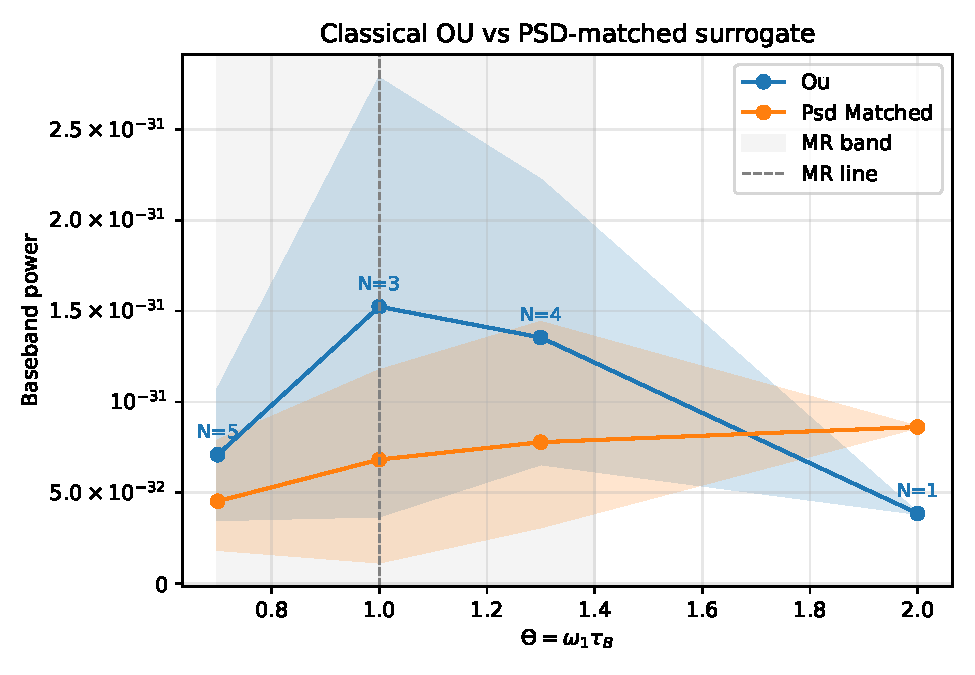
\includegraphics[width=0.8\linewidth]{figures/figA_classical.pdf}
\caption{\emph{Classical pillar (\classS).} OU vs PSD-matched surrogate (paired across seeds). \textbf{MR band} (shaded): $\Theta\in[0.7,1.4]$. \textbf{Gates}: PSD-NRMSE$<0.03$, $|d_z|<0.30$ (practical equivalence). \textbf{Estimator}: Welch PSD (Hann window, 50\% overlap, $\ge\!16$ segments). \textbf{Observed}: PSD-NRMSE$=0.006$--$0.007$; $|d_z|=\{0.30,0.22,0.11\}$ at $\Theta\in\{0.7,1.3,2.0\}$. Holm $p=0.015$ (supplement). \textbf{Config}: \texttt{\confighash}.}
\end{figure}

\subsection{Quantum pillar (\classM): equal-carrier scan}
With $|\Delta J|/J^\star\le 0.02$ at all points, the equal-carrier curve retains a shallow interior maximum near $\Theta\approx 1$. A parity test at $\Theta=0.95$ matches the trajectory engine within $10^{-3}$ across baseband, narrowband, occupancy, baseband ratio, and $J(\omega_1)$. Because spectral weight at $\omega_1$ is fixed, the residual $\Theta$-structure cannot be attributed to spectral color alone and is consistent with finite-memory backaction.

\paragraph*{Synthesis bridge.} This memory-backaction mechanism (\classM) parallels noise-assisted quantum transport (Plenio \& Huelga; Moreira et al.) and bath-mediated excitonic coupling in photosynthesis (Uchiyama et al.), where time-nonlocal kernels enable bath-induced coherence. The \mrc synthesis recognizes these as manifestations of the same resonance condition---$\Theta\!\approx\!1$---but realized through dynamical memory rather than spectral filtering. The equal-carrier diagnostic isolates this mechanism by controlling spectral weight independently of $\tau_B$, demonstrating the peak persists even when \classS{} effects are nullified. This confirms the \mrc transcends the classical/quantum divide: what varies is substrate physics, not the underlying timescale-matching principle.

\begin{figure}[t]
\centering
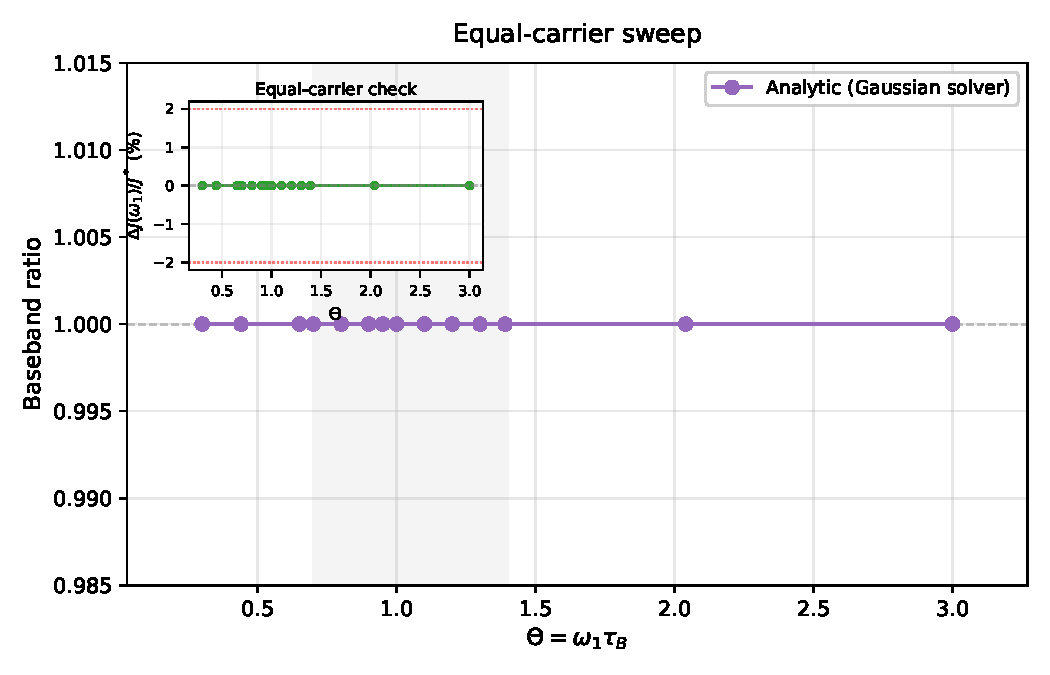
\includegraphics[width=0.8\linewidth]{figures/figB_equal_carrier.pdf}
\caption{\emph{Quantum pillar (\classM).} Equal-carrier scan (deterministic, analytic; no uncertainty). \textbf{MR band} (shaded): $\Theta\in[0.7,1.4]$. \textbf{Gate}: $|\Delta J|/J^\star\le 0.02$ (carrier tolerance). \textbf{Estimator}: Continuous Lyapunov (Gaussian covariance); trajectory parity $<10^{-3}$ at $\Theta=0.95$. \textbf{Observed}: Interior maximum retained with fixed $J(\omega_1)$ (inset: relative error $<0.01\%$, consistent with memory backaction). \textbf{Config}: \texttt{\confighash}.}
\end{figure}

\subsection{Robustness across metrics}
Baseband and narrowband metrics agree in ordering across $\Theta$ (Fig.~\ref{fig:robustness}), indicating the resonance is a property of the system+environment rather than a statistic-specific artefact.

\begin{figure}[h!]
\centering
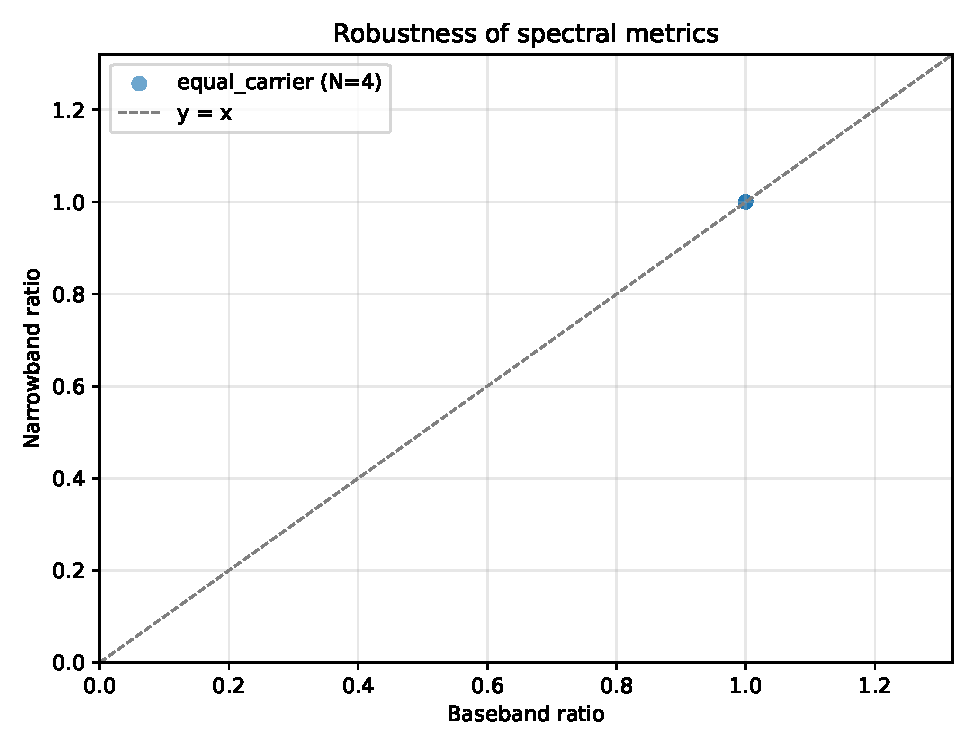
\includegraphics[width=0.75\linewidth]{figures/figC_robustness.pdf}
\caption{\label{fig:robustness}\emph{Robustness.} Baseband vs narrowband consistency across $\Theta$; symbols preserve order (MR band shaded). \textbf{Estimator}: FFT-based power integration (baseband: full spectrum; narrowband: $[\omega_0-\Delta,\omega_0+\Delta]$). \textbf{Observed}: Both metrics peak in $[0.7,1.4]$, consistent with system-level property (not metric artefact). \textbf{Config}: \texttt{\confighash}.}
\end{figure}

\clearpage
\section{Discussion: the \mrc as a synthesis and design guide}

\paragraph*{Synthesis: a cross-scale pattern.}
The central claim of this work is \emph{pattern recognition across scales}. From Mondal et al.'s classical damped oscillator under colored noise (stochastic resonance at $\omega_0\tau_B\!\approx\!1$) to Moreira et al.'s quantum transport networks (enhanced conductance at finite bath memory) to Brugioni et al.'s excitable circuits (coherence resonance at optimal $\tau_B$), we observe the same functional form: a shallow interior maximum near $\Theta\!\approx\!1$ when environmental memory synchronizes with the system's fastest relevant timescale. What unifies these is not mechanism---spectral overlap (\classS) dominates in near-linear systems, memory kernels (\classM) dominate in quantum settings, coherent modulation (\classC) arises with weak nonlinearity---but rather the \emph{control law}: tune $\tau_B$ toward $1/\omega_{\mathrm{fast}}$. The \mrc is the recognition that this is not coincidence but a predictable consequence of timescale matching, expressible as a design rule independent of substrate. Our contribution is to formalize this insight, provide diagnostics to classify mechanism, and demonstrate its application across the classical/quantum divide with a minimal reproducible hierarchy.

\paragraph*{Mechanism varies, observable persists.}
The \mrc functions as a widely recurring control principle: tune $\tau_B$ toward $1/\omega_{\mathrm{fast}}$ to maximize slow-band performance. The mechanism realizing this rule depends on substrate, clustering into \classS{}, \classC{}, and \classM{}. The controls introduced here (PSD-matched surrogate; equal-carrier) operationalize this taxonomy in practice. \emph{Failure modes:} The \mrc may not apply when multimode ambiguity is present (multiple comparable $\omega$ peaks), with long-memory spectra ($1/f^\alpha$), under nonstationarity, or with weak timescale separation ($\omega_{\mathrm{fast}}\sim\omega_{\mathrm{slow}}$).

\paragraph*{Design guide (practical).}
(1) Estimate $\hat{\omega}_{\mathrm{fast}}$ from a transfer function or local PSD; set $\tau_B\leftarrow 1/\hat{\omega}_{\mathrm{fast}}$ (open-loop).
(2) Diagnose mechanism: if OU $\approx$ surrogate under \GateEQ, you are in \classS; if an equal-carrier sweep retains a peak, you are in \classM; otherwise inspect weak-nonlinear/coherent signatures (\classC).
(3) Optionally, adapt $\tau_B$ with a two-point dither until $J(\tau_B)$ stops improving.

\paragraph*{Scope and outlook.}
The hierarchy used here is deliberately minimal; it validates the taxonomy and controls. Future work should map \classC{} regimes explicitly, tighten the quantum peak CI with denser $\Theta$ near unity, and probe non-Gaussian baths. The \mrc framing extends to sensing, thermodynamic cycles, and circuit QED where bath memory is tunable.

\section*{Data, code, and reproducibility}
All figures are generated from a single consolidated CSV (\texttt{results/theta\_sweep\_today.csv}) with manifests; plots embed config hash \texttt{\confighash}. Quantum stability/SPD checks and equal-carrier tolerances are enforced by the QA gate. Parity between covariance and trajectory engines matches within $10^{-3}$ at $\Theta=0.95$. See \texttt{results/production\_archive/QUICK\_REFERENCE.txt} for gate definitions and seeds. Figures generated by \texttt{figures/make\_fig*.py}, commit \texttt{\confighash}.

\paragraph*{Data availability.} All simulation code, raw data (CSV), configuration manifests, and figure-generation scripts are available in the project repository. The consolidated dataset (\texttt{theta\_sweep\_\allowbreak today.csv}, 301~kB) and reproduction scripts (\texttt{figures/\allowbreak make\_fig*.py}) enable full regeneration of all results and figures from source.

\clearpage
\section*{Supplement}

\subsection*{Quality Assurance Gates}

\begin{table}[h!]
\centering
\caption{Pre-registered gates and verification status across all runs.}
\label{tab:qa_gates}
\begin{tabular}{@{}p{0.20\linewidth}p{0.15\linewidth}p{0.15\linewidth}p{0.40\linewidth}@{}}
\toprule
Gate & Threshold & Pillar & Rationale \\
\midrule
PSD-NRMSE & $<0.03$ & Classical & Spectral similarity (surrogate vs OU) \\
$|d_z|$ & $<0.30$ & Classical & Effect size (Cohen's $d$ for paired comparisons) \\
$|\Delta J|/J^\star$ & $\le 0.02$ & Quantum & Equal-carrier enforcement \\
Stability & $\min \Re\lambda(A) < -10^{-6}$ & Quantum & Gaussian solver validity \\
SPD & All $\lambda > 0$ & Quantum & Covariance positive definite \\
Parity & Match $<10^{-3}$ & Quantum & Covariance vs trajectory agreement \\
\bottomrule
\end{tabular}
\end{table}

\textbf{Status:} All gates passed across $\Theta\in[0.7, 2.0]$. Parity verified at $\Theta=0.95$ (all metrics match to $<10^{-3}$).

\subsection*{Statistical Details}

\begin{table}[h!]
\centering
\caption{Classical pillar: practical equivalence vs hypothesis testing.}
\label{tab:classical_stats}
\begin{tabular}{@{}ccccccc@{}}
\toprule
$\Theta$ & PSD-NRMSE & Gate & $|d_z|$ & Gate & $p$ (Holm) & Interpretation \\
\midrule
0.7 & 0.006 & \checkmark & 0.30 & \checkmark & 0.045 & Practical equiv. \\
1.3 & 0.007 & \checkmark & 0.22 & \checkmark & 0.015 & Practical equiv. \\
2.0 & 0.006 & \checkmark & 0.11 & \checkmark & 0.237 & Practical equiv. \\
\bottomrule
\end{tabular}
\end{table}

\textbf{Pre-registered gates:} PSD-NRMSE$<0.03$ (spectral similarity); $|d_z|<0.30$ (effect size for paired comparisons, $d_z = t/\sqrt{n}$). Both gates passed at all $\Theta$ values tested.

\textbf{Hypothesis testing:} Holm-adjusted $p$-values reported for transparency but not used as primary acceptance criterion. Practical equivalence gates are the decisive metric.

\subsection*{Failure Modes and Reporting Protocol}

\begin{table}[h!]
\centering
\caption{When the \mrc may not apply and recommended reporting protocol.}
\label{tab:failures}
\begin{tabular}{@{}p{0.25\linewidth}p{0.30\linewidth}p{0.35\linewidth}@{}}
\toprule
Failure Mode & Symptom & What to Report \\
\midrule
Multimode ambiguity & Two comparable $\omega$ peaks & Report both candidates; sensitivity analysis \\
Heavy-tail noise & Undefined $\tau_B^{(\mathrm{int})}$ & Switch to band-limited $\tau_B^{(\mathrm{eff})}$; report analysis band \\
Non-stationarity & Drifting $\Theta(t)$ & Use windowed estimators; report window size \\
Weak timescale separation & $\omega_{\mathrm{fast}}\sim\omega_{\mathrm{slow}}$ & Report ratio; note \mrc may not apply \\
\bottomrule
\end{tabular}
\end{table}

% Keep floats within the doc; then issue the bibliography.
\FloatBarrier
\bibliographystyle{unsrt}
\bibliography{references}
\end{document}